\documentclass[11pt]{article}
\usepackage[utf8]{inputenc}
\usepackage[T1]{fontenc}
\usepackage{amsmath}
\usepackage{amssymb} % Needed for \eth
\usepackage{graphicx}
\usepackage{geometry}
\usepackage{tikz}
\usepackage{ulem}     % For underline, using normalem to avoid messing with \emph

\geometry{a4paper, margin=1in}
\usetikzlibrary{positioning, arrows.meta, shapes.geometric, patterns} % For TikZ diagrams

% Custom commands (optional)
\newcommand{\avg}[1]{\overline{#1}}
\newcommand{\prob}[1]{P(#1)}
\newcommand{\ProbDens}[1]{\mathcal{P}(#1)} % Using script P for density
\newcommand{\vect}[1]{\vec{#1}}
\newcommand{\dd}[1]{\mathrm{d}#1} % Differential d
\newcommand{\pderiv}[2]{\frac{\partial #1}{\partial #2}}
\newcommand{\deriv}[2]{\frac{\mathrm{d} #1}{\mathrm{d} #2}}
\newcommand{\muState}{\mu\text{-state}} % Microstate
\newcommand{\OmegaE}{\Omega(E)}
\newcommand{\omegaE}{\omega(E)}
\newcommand{\PhiE}{\Phi(E)}
\newcommand{\deltaE}{\delta E}
\newcommand{\ethbar}{\text{\it{đ}}} % \eth symbol for inexact differential

\title{Physics 415 - Lecture 5: Interaction Between Macroscopic Bodies}
\date{January 31, 2025}
\author{} % Author not specified

\begin{document}

\maketitle
\thispagestyle{empty}

\section*{Summary}

\begin{itemize}
    \item Statistical description of systems of particles:
    \begin{itemize}
        \item Classical: $\muState \leftrightarrow$ phase space cell (size $h_0^S$).
        \item Quantum: $\muState \leftrightarrow$ quantum state specified by $f$ quantum numbers $\{n_1, \dots, n_f\}$.
    \end{itemize}
    \item $\OmegaE = $ \# of accessible states $\sim E^{Na}$ ($N=$ \# of particles, $a \sim O(1)$).
    \item Fundamental postulate: Prob($\muState$) $= 1/\OmegaE$ for accessible states.
\end{itemize}

\section*{Interaction Between Macroscopic Bodies}

Consider a macroscopic system whose Hamiltonian depends on some external parameters $x_1, x_2, \dots, x_n$:
\[ H = H(q, p; x_1, \dots, x_n) \quad (\text{CM or QM}) \]
Examples of external parameters $x_k$:
\begin{itemize}
    \item $x = V =$ volume of the system.
    \item $x =$ externally applied field ($\mathcal{E}$, $B$, etc.).
\end{itemize}
The energy levels $E_r$ of the system also depend on these parameters:
\[ E_r = E_r(x_1, x_2, \dots, x_n) \quad (\text{CM or QM}) \]
A "macrostate" of the system is defined by specifying the values of all external parameters $(x_1, \dots, x_n)$ and any other condition specified on the system, like the total energy $E$.
\textbf{Example:} A system with fixed volume $V$ and fixed total energy $E$.

In a statistical ensemble, all $\mathcal{N}$ members are prepared in accordance with the specification of the macrostate.
\textbf{Example:} All members have the same volume $V$ and total energy $E$ (or energy in range $(E, E+\deltaE)$).
For a given macrostate, the system can be in any one of a very large number ($\OmegaE$) of accessible $\mu$-states.
Note the difference:
\begin{itemize}
    \item Data to specify macrostate $<<$ Data to specify $\mu$-state.
\end{itemize}

Consider now two macroscopic systems A \& B that can interact with each other, such that the total energy $E_{total} = E_A + E_B$ is conserved.
We distinguish two types of interaction:

\subsection*{1) Thermal Interaction}

\begin{itemize}
    \item Systems can exchange energy.
    \item External parameters are fixed, so energy levels $E_r^{(A)}$ and $E_r^{(B)}$ do not change. (This description uses QM language, but applies to CM too).
    \item Energy is transferred from one system to the other.
\end{itemize}

Consider the statistical ensemble.
\begin{itemize}
    \item When thermal interaction is "turned off" (initially or conceptually), system A has energy $E_A^{(i)}$ and B has $E_B^{(i)}$ for member $i$ of the ensemble. $E_A^{(i)} + E_B^{(i)} = E = \text{const}$.
    \item With thermal interaction allowed, after the combined system (A+B) has come to equilibrium, energy may have been transferred. For member $i$, let $\Delta E_i$ be the energy transferred from B to A.
    \item The final energies are $E_A^{\prime (i)} = E_A^{(i)} + \Delta E_i$ and $E_B^{\prime (i)} = E_B^{(i)} - \Delta E_i$.
    \item There will be a distribution of $\Delta E_i$ across the ensemble.
\end{itemize}
We consider the mean energy transfer $\avg{\Delta E}$. This is defined as the "heat" $Q$ absorbed by system A:
\[ Q_A = \avg{\Delta E} \]
If $\avg{\Delta E} > 0$, A absorbs heat. If $\avg{\Delta E} < 0$, A gives off heat.
(Heat absorbed by A = Heat given off by B, and vice-versa, since $E_A+E_B$ is constant).

Later we'll see that the distribution of $\Delta E_i$ is typically very sharply peaked about the mean $\avg{\Delta E}$ for macroscopic systems, so that statistical fluctuations will be entirely negligible. The same will be true for most macroscopic properties.

\subsection*{2) Mechanical Interaction}

Consider "thermally isolated" systems (no thermal interaction with each other or the environment).
Two thermally isolated systems may still interact through changes in their external parameters. This is "mechanical interaction".
In this case, systems exchange energy through "macroscopic work".

\textbf{Example:} Gas expanding against a piston connected to a weight.

\begin{center}
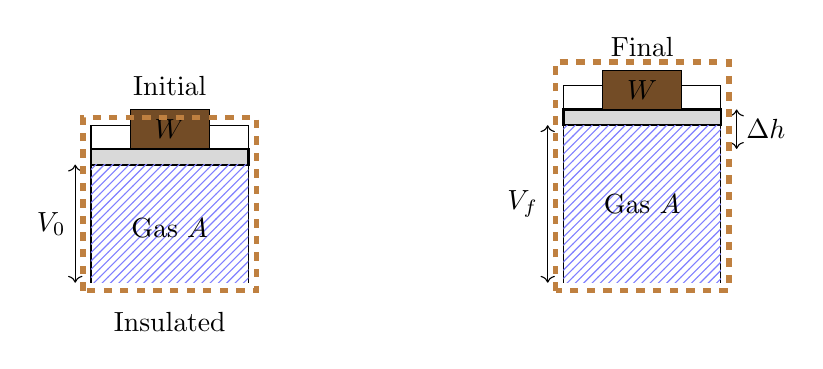
\begin{tikzpicture}
    % Initial State
    \begin{scope}[xshift=-3cm]
        \node at (0, 2.5) {Initial};
        % Cylinder
        \draw (-1,0) -- (-1,2) -- (1,2) -- (1,0);
        % Piston
        \draw[thick, fill=gray!30] (-1, 1.5) rectangle (1, 1.7);
        % Weight
        \draw[fill=brown!60!black] (-0.5, 1.7) rectangle (0.5, 2.2);
        \node at (0, 1.95) {$W$};
        % Gas
        \fill [pattern=north east lines, pattern color=blue!50] (-1,0) rectangle (1, 1.5);
        \node at (0, 0.7) {Gas $A$};
        % Label V0
        \draw[<->] (-1.2, 0) -- (-1.2, 1.5) node[midway, left] {$V_0$};
        % Insulation
        \draw[line width=2pt, brown, dashed] (-1.1, -0.1) rectangle (1.1, 2.1);
        \node at (0, -0.5) {Insulated};
    \end{scope}

    % Final State
    \begin{scope}[xshift=3cm]
        \node at (0, 3) {Final};
        % Cylinder
        \draw (-1,0) -- (-1,2.5) -- (1,2.5) -- (1,0); % Taller cylinder space
        % Piston (moved up)
        \draw[thick, fill=gray!30] (-1, 2.0) rectangle (1, 2.2);
        % Weight (moved up)
        \draw[fill=brown!60!black] (-0.5, 2.2) rectangle (0.5, 2.7);
        \node at (0, 2.45) {$W$};
        % Gas (expanded)
        \fill [pattern=north east lines, pattern color=blue!50] (-1,0) rectangle (1, 2.0);
        \node at (0, 1) {Gas $A$};
        % Label Vf
        \draw[<->] (-1.2, 0) -- (-1.2, 2.0) node[midway, left] {$V_f$};
        % Label dh
        \draw[<->] (1.2, 1.7) -- (1.2, 2.2) node[midway, right] {$\Delta h$};
        % Insulation
        \draw[line width=2pt, brown, dashed] (-1.1, -0.1) rectangle (1.1, 2.8);
    \end{scope}
\end{tikzpicture}
\end{center}

\begin{itemize}
    \item System A = Gas, System B = Weight + Piston.
    \item Initially compressed gas. Gas expands, raising weight by amount $\Delta h$.
    \item Gas (A) does work raising weight + piston (B).
    \item Change in external parameters: Change in volume for A ($V_0 \to V_f$) and change in height for B ($\Delta h$).
    \item The work done *by* the gas (neglecting weight of piston) is simply $W_{by A} = (\text{weight}) \times \Delta h$.
\end{itemize}

In the language of the statistical ensemble:
As an external parameter $x_\alpha$ is varied, the energy of system $i$ changes by an amount $\Delta_{x_\alpha} E^{(i)}$.
Consider the mean change $\avg{\Delta_{x_\alpha} E}$. This quantity is the "macroscopic work" done *on* the system A.
\[ W_{on A} = \avg{\Delta_x E} \]
% Note: The subscript x indicates change due to external parameter variation.
We will more often use the quantity $W =$ work done *by* the system.
\[ W = -W_{on A} = -\avg{\Delta_x E} \]
In the example of the gas and weight+piston, $W_{by A} = (\text{weight}) \times \Delta h$.

\section*{First Law of Thermodynamics}

In general, interaction between systems involves both a change in their external parameters (mechanical interaction) and heat exchange if they are not thermally isolated (thermal interaction).
As a result of such an interaction, the mean energy of system A will be changed by an amount $\Delta \avg{E}$.

If $\avg{\Delta_x E} = -W$ is the increase in mean energy from macroscopic work done *on* the system, then we write the total change in energy as:
\[ \Delta \avg{E} = \avg{\Delta_x E} + Q \]
This relation defines the heat $Q$ absorbed by system A:
\[ Q \equiv \Delta \avg{E} - \avg{\Delta_x E} = \Delta \avg{E} + W \]

\begin{itemize}
    \item $Q$ = Mean energy change not due to change in external parameters (i.e., not due to macro work). It represents energy transfer due to microscopic degrees of freedom (thermal interaction).
    \item $\Delta \avg{E}$ = Total change in mean internal energy of system A.
    \item $W$ = Macroscopic work done *by* system A.
\end{itemize}
This is the First Law of Thermodynamics: The change in the internal energy of a system is equal to the heat added to the system minus the work done by the system ($\Delta \avg{E} = Q - W$, which is equivalent to $Q = \Delta \avg{E} + W$).

\textbf{Example:} If the piston in the previous example is not insulating and is free to move, both mechanical and thermal interaction occurs between A \& B.

When the work done by the system is small (infinitesimal), $\ethbar W$, and correspondingly the change in mean energy is small, $d\avg{E}$, we write the first law in differential form:
\[ \ethbar Q \equiv d\avg{E} + \ethbar W \]
\begin{itemize}
    \item $\ethbar W$ = small work done *by* the system.
    \item $\ethbar Q$ = small amount of heat absorbed *by* the system.
    \item The symbol $\ethbar$ (or often $\delta$) denotes an "inexact" differential.
    \item Unlike the usual "d", $\ethbar$ does not indicate a small change in the value of a state function. While $d\avg{E}$ is a small difference between values of mean energy (a state function), there is no meaning to "small difference between works/heats".
    \item Moreover, while the mean energy $\avg{E}$ of a system is a well-defined quantity for a system in a given state, there is no meaning to "quantity of heat/work" contained in the system in a given state. Heat and Work are processes of energy transfer, not properties of the state itself.
\end{itemize}

\end{document}